\chapter{马尔可夫随机场}

\textsl{马尔可夫随机场(Markov Random Field,简称 MRF)}是一种\textsl{无向图模型},图中每一个结点
表示一个或者一组变量,结点之间的边表示两个变量之间的依赖关系。马尔科夫随机场又一组\textsl{势函数(potential function)},
也称为\textsl{因子(factor)},这是定义在变量子集上的非负实函数,主要用于定义概率分布函数。

\section{极大团}

下图是一个简单的马尔可夫随机场,对于图中结点的一个子集,如果任意两个结点之间有边链接,则称该节点子集为一个\textbf{团(clique)},
若在一个团中加入另外任意一个结点都不在形成团,则该团称为\textbf{极大团(maximal clique)}。即\textsl{极大团就是不能被其他团所包含的团}。

\begin{figure}[H]
    \centering
    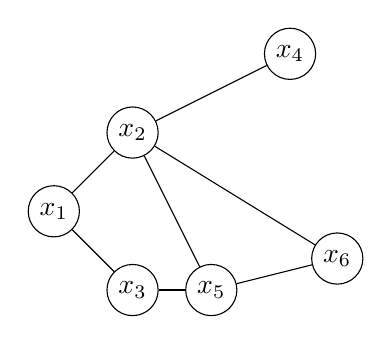
\begin{tikzpicture}
        \node[circle,draw = black,fill = white,inner sep = 0pt,minimum size = 0.65cm] (x1) at (0, 0)  {{$x_1$}};
        \node[circle,draw = black,fill = white,inner sep = 0pt,minimum size = 0.65cm] (x2) at (1, 1) {{$x_2$}};
        \node[circle,draw = black,fill = white,inner sep = 0pt,minimum size = 0.65cm] (x3) at (1, -1)  {{$x_3$}};
        \node[circle,draw = black,fill = white,inner sep = 0pt,minimum size = 0.65cm] (x4) at (3, 2)  {{$x_4$}};
        \node[circle,draw = black,fill = white,inner sep = 0pt,minimum size = 0.65cm] (x5) at (2, -1)  {{$x_5$}};
        \node[circle,draw = black,fill = white,inner sep = 0pt,minimum size = 0.65cm] (x6) at (3.6, -0.6)  {{$x_6$}};
        \path[draw,-] (x1) edge (x2);
        \path[draw,-] (x1) edge (x3);
        \path[draw,-] (x2) edge (x4);
        \path[draw,-] (x2) edge (x5);
        \path[draw,-] (x3) edge (x5);
        \path[draw,-] (x5) edge (x6);
        \path[draw,-] (x2) edge (x6);
    \end{tikzpicture}
    \caption{一个简单的马尔可夫随机场例子}
    \label{一个简单的马尔可夫随机场例子}
\end{figure}

上例中,$\{x_1,x_2\}$,$\{x_1,x_3\}$,$\{x_3,x_5\}$,$\{x_2,x_5\}$,$\{x_2,x_6\}$,$\{x_5,x_6\}$,$\{x_2,x_4\}$和$\{x_2,x_5,x_6\}$都是团,但是除了
$\{x_2,x_5\}$,$\{x_2,x_6\}$,$\{x_5,x_6\}$,以外都是极大团。显然,每个节点至少出现在一个极大团中。

\section{联合概率}

\subsection*{无向图的联合概率表示}

在马尔可夫随机场中,多个变量之间的联合概率分布能基于团分解为多个因子的乘积,\textbf{每个因子仅仅只和一个团相关},具体来说,对于$n$个变量$x=\{x_1,x_2,\cdots,x_n\}$,所有团构成集合$\mathcal{C}$,
与团$\mathcal{Q}\in \mathcal{C}$对应的变量集合记为$x_Q$,则联合概率$P(x)$定义为
\begin{equation}
    P(x)=\frac{1}{Z}\prod\limits_{\mathcal{Q}\in \mathcal{C}}\psi_Q(x_Q)
\end{equation}

其中$\psi_Q$为与团对应的是势函数,用于对团$\mathcal{Q}$中的变量关系进行建模,$Z$为规范化因子,以确保$P(x)$定义的概率是有意义的,表达式如下
\begin{equation}
    Z=\sum_{x}\prod_{\mathcal{Q}\in \mathcal{C}}\psi_Q(x_Q)
\end{equation}

\subsection*{基于极大团定义联合概率}

显然如果变量比较多,那么团的数量就会很多,这就意味着联合概率就会有很多乘积项,显然会给计算带来负担,但是我们注意到
\textsl{如果$\mathcal{Q}$不是最大团,那么它势必会被一个极大团$\mathcal{Q}^*$所包含,这意味着变量$x_Q$之间的关系不仅体现在势函数$\psi_Q$中,函体现在$\psi_{Q^*}$}。于是
由极大团来定义联合概率,假定所有极大团构成的集合为$\mathcal{C}^*$,则
\begin{equation}
    P(x)=\frac{1}{Z^*}\prod\limits_{\mathcal{Q}\in \mathcal{C}^*}\psi_{Q^*}(x_{Q^*})
\end{equation}

这样来说我们就不需要去统计每个团的势函数的积。

\begin{figure}[H]
    \centering
    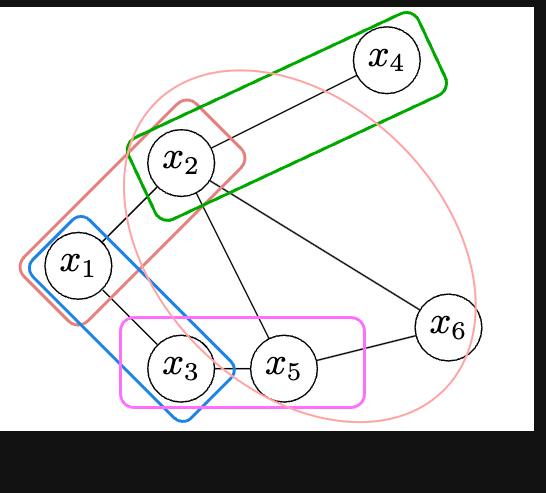
\includegraphics[scale=0.5]{figures/基于极大团的联合概率分布.png}
    \caption{基于极大团的联合概率分布}
\end{figure}

\section{条件独立性}

在马尔可夫随机场中如何得到条件独立性呢?同样借助“分离”的概念,如下图所示,如果结点集$A$的结点到$B$中的结点都必须经过结点集$C$中的结点,
则称结点集$A$和$B$被结点集$C$分离,$C$称为\textsl{分离集}。

\begin{figure}[H]
    \centering
    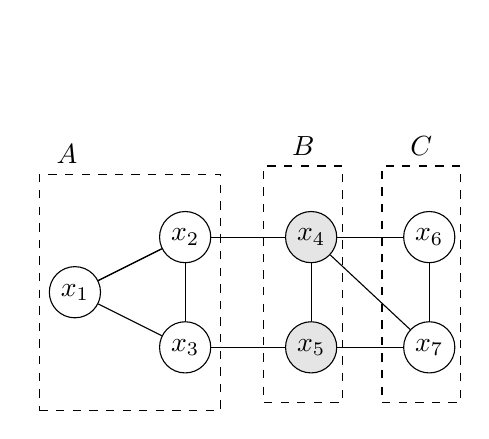
\begin{tikzpicture}
        \node[circle,draw = black,fill = white,inner sep = 0pt,minimum size = 0.65cm] (x1) at (0, 0)  {{$x_1$}};
        \node[circle,draw = black,fill = white,inner sep = 0pt,minimum size = 0.65cm] (x2) at (1.4, 0.7) {{$x_2$}};
        \node[circle,draw = black,fill = white,inner sep = 0pt,minimum size = 0.65cm] (x3) at (1.4, -0.7)  {{$x_3$}};
        \node[circle,draw = black,fill = gray!20,inner sep = 0pt,minimum size = 0.65cm] (x4) at (3.0, 0.7)  {{$x_4$}};
        \node[circle,draw = black,fill = gray!20,inner sep = 0pt,minimum size = 0.65cm] (x5) at (3.0, -0.7)  {{$x_5$}};
        \node[circle,draw = black,fill = white,inner sep = 0pt,minimum size = 0.65cm] (x6) at (4.5, 0.7)  {{$x_6$}};
        \node[circle,draw = black,fill = white,inner sep = 0pt,minimum size = 0.65cm] (x7) at (4.5, -0.7)  {{$x_7$}};
        \node[draw, dashed, rectangle, minimum width=2.3cm, minimum height=3cm,xshift=0.7cm] at (x1.center) {};
        \node[draw, dashed, rectangle, minimum width=1cm, minimum height=3cm,xshift=-0.1cm,yshift=-17] at (x4.center) {};
        \node[draw, dashed, rectangle, minimum width=1cm, minimum height=3cm,xshift=-0.1cm,yshift=-17] at (x6.center) {};
        \node[draw=none, rectangle, minimum width=1cm, minimum height=3cm,xshift=-0.1cm,yshift=50] at (x1.center) {$A$};
        \node[draw=none, rectangle, minimum width=1cm, minimum height=3cm,xshift=-0.1cm,yshift=33] at (x4.center) {$B$};
        \node[draw=none, rectangle, minimum width=1cm, minimum height=3cm,xshift=-0.1cm,yshift=33] at (x6.center) {$C$};
        \path[draw,-] (x1) edge (x2);
        \path[draw,-] (x1) edge (x3);
        \path[draw,-] (x3) edge (x2);
        \path[draw,-] (x3) edge (x5);
        \path[draw,-] (x2) edge (x4);
        \path[draw,-] (x1) edge (x2);
        \path[draw,-] (x4) edge (x6);
        \path[draw,-] (x5) edge (x7);
        \path[draw,-] (x6) edge (x7);
        \path[draw,-] (x4) edge (x5);
        \path[draw,-] (x4) edge (x7);
    \end{tikzpicture}
    \caption{$x_4$和$x_5$组成的团是分离集}
\end{figure}



\subsection*{全局马尔可夫}

给给定两个变量的子集的分离集,则这两个子集条件独立。

\subsection*{局部马尔可夫}

给定某变量的邻接变量,则该变量条件独立于其他变量,形式地说,令$V$为图的结点集合,$n(v)$为结点$v$在图上的邻接结点,$n^*(v)=n(v)\cup\{v\}$,有
$x_v\perp x_{V/n^*(v)}|x_n(v)$。

\subsection*{成对马尔可夫}

给定某变量的邻接变量,两个非邻接变量条件独立,形式化地说,令图的结点集和边集分别为$V$和$E$,对途中两个结点$u$和$v$,
若$\left\langle u,v\right\rangle \notin E$,则$x_u\perp x_{V/\left\langle u,v\right\rangle}$

\begin{proposition}
    三种马尔可夫是相互等价的
\end{proposition}

\section{因式分解与Hammesley-Clifford 定理}

\begin{define}
    (团) 团是一个关于节点的集合,集合中的节点之间相互都是连通的(都有边)。
\end{define}

\begin{define}
    (最大团) 团中没办法添进去新的节点。
\end{define}

基于最大团形式的因式分解。
\begin{equation}
    p(x)=\frac{1}{z}\prod\limits_{i=1}^{K}\varphi(x_{ci})
\end{equation}

其中$c_i$是最大团,$x_{ci}$最大团随机变量集合,$\varphi(x_{ci})$势函数,必须为正。

有一个定理保证基于最大团的因式分解是马尔可夫随机场

\begin{theorem}
    (Hammesley-Clifford 定理)
\end{theorem}

Markov Random Field $\Leftrightarrow$ Gibbs Distribution

吉布斯概率分布和玻尔兹曼分布
(这部分最好提前去了解一下统计物理里面的概念)

吉布斯分布在概率分布的角度还具备了最大熵的概念。

马尔可夫随机场

\section{马尔可夫随机场中的势函数}

势函数用来定量刻画变量集$x_Q$中变量之间的相关关系,他应该是非负函数,且在所偏好的变量取值上有较大函数值。例如
\begin{equation}
    \psi_{AC}(x_A,x_C)=
    \begin{cases}
        & 1.5,\ \ \ \ if\ x_A=x_C\\
        & 0.1,\ \ \ \ ohterwise
    \end{cases}
    \nonumber
\end{equation}

\begin{equation}
    \psi_{BC}(x_B,x_C)=
    \begin{cases}
        & 0.2,\ \ \ \ if\ x_B=x_C\\
        & 1.3,\ \ \ \ ohterwise
    \end{cases}
    \nonumber
\end{equation}

则说明该模型偏好变量$x_A$和$x_C$有相同的取值,$x_B$和$x_C$有不同的取值。换言之$x_A$和$x_C$正相关,$x_B$和$x_C$负相关。

常用的势函数还有指数函数
\begin{equation}
    \psi_Q(x_Q)=e^{-H_Q(x_Q)}
\end{equation}